\chapter{Implementation}
\label{cha:implementierung}

\section{System Architecture}

The system architecture, depicted in figure xx, integrates the behavior tree, responsible for the behavior planning, in a position to override Navigation2. This is done through the help of the Decision Gate, that can selectively forward speed commands to the robot controller. 
The behavior tree can access the sensor data when needed through the Data Backup component. The System Supervision component controls the health of all components, but the connections are not depicted in the component diagram for Übersichtlichkeit.

\begin{figure}[h!]
	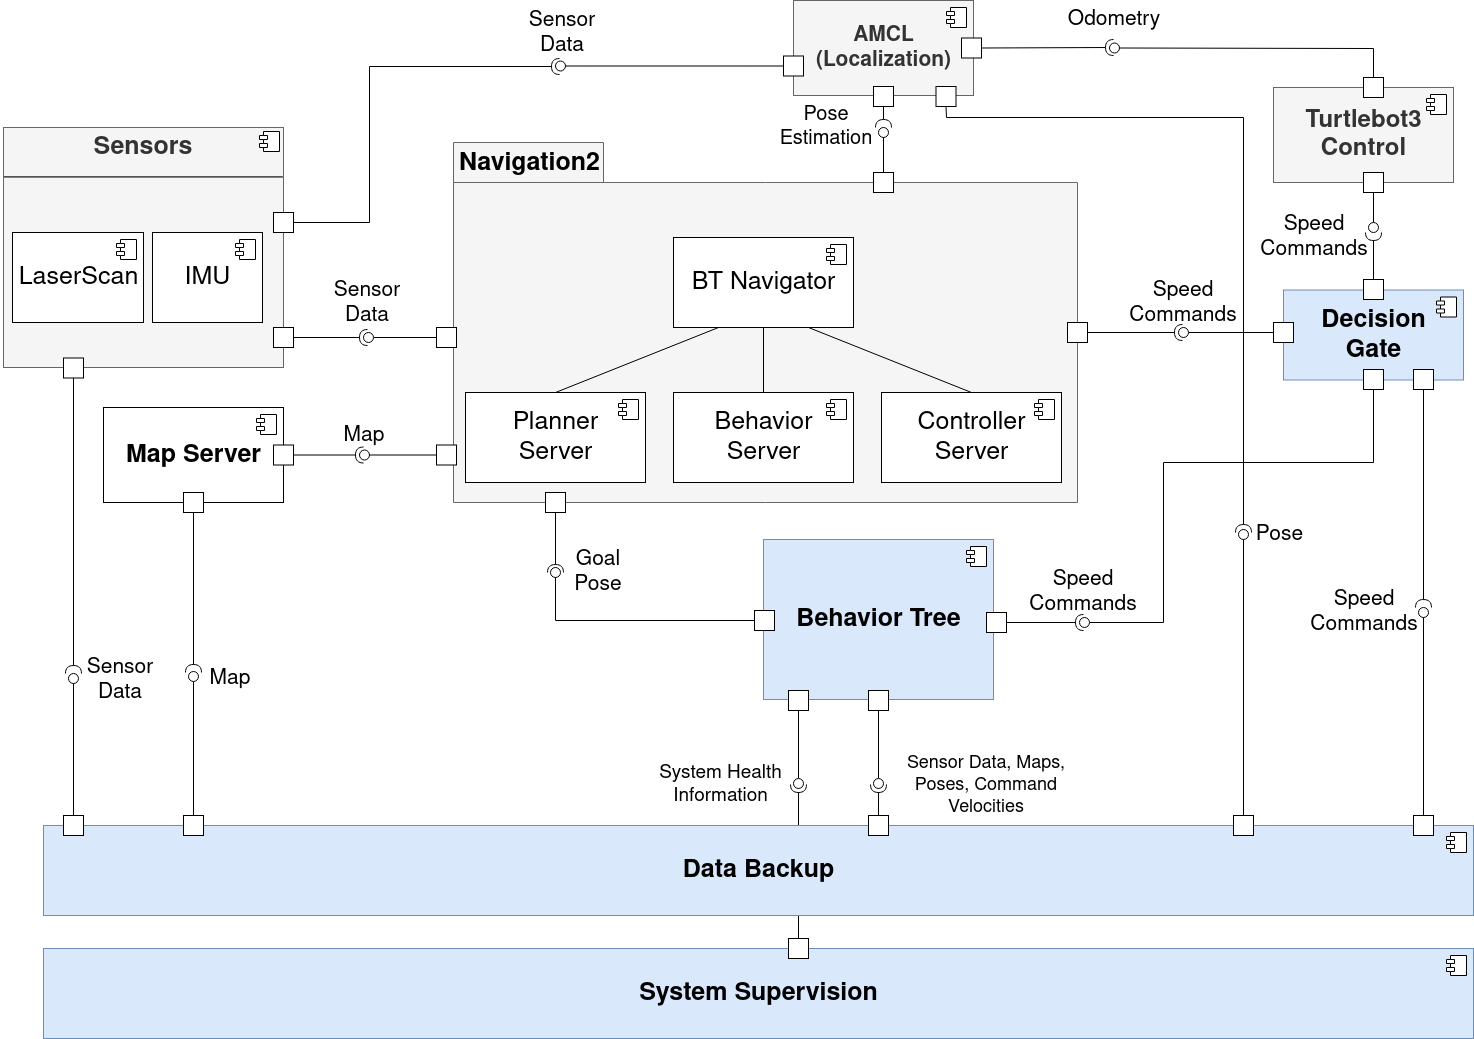
\includegraphics[width=1.05\textwidth]{images/component_diagram_bt.png}
	\caption{Component Diagram of System Architecture}
\end{figure}

\section{Data Backup}
The data backup component functions as a way to efficiently gather data from all components of the system and bereitstellen necessary data to the behavior tree when the planning process requires the use of past data points.  This component subscribes is a to all sensor data and saves the messages in a queue data structure. The most recent data gets pushed into the array and if the array exceeds a bestimmte length, the oldest data this data gets deleted from the array. The limited array size is twofold. On the on side, the goal is to decrease the size of the message that gets sent to the BT to limit the network auslastung and on the other side, the BT often does not need to look back further than a few seconds to make a decision. This way the computational load and network load is decreased.
The BT can access the saved data by sending a service call to one of the provided services by this component. Service calls in ROS2 are executed with hihg priority and the execution is done quickly but it adds an additional step than just saving the data directly in the behavior tree. The reason for the outsourcing of the data backup in another component is that ROS node need an executor which spins the node constantly. The spinning allows the node to check the network if there is any work to do for the node. This means that if one of the subscribed topic received a message, the node has to execute one of its callback functions that is associated with that topic. This spinning has to be done in regular intervals, otherwise the node might miss incoming messages from subscribed topics. The way to do the spinning is to have the node spun constantly in one thread. Have a constant spinning node would block the execution of the BT completely. If one would try to spin a node once when a node gets ticked in the BT, the problem of missing messages would become relevant because the BT might need longer than exepected to return to a node to tick it. That way the BT node that would be responsible for saving all the relevant data can not guarantee that it has picked up on all of the messages between to spins. The synchronous nature of the ROS executor spinning the nodes is the reason why the data backup is not stored within the BT. 

The saved data inside of this component with the corresponding lookback time is listed in table xx. 

\begin{table}[h!]
	\caption{Types of saved data}
	\begin{tabular}{ | m{0.2\textwidth} | m{0.25\textwidth}| m{0.25\textwidth} | m{0.2\textwidth} |} 
  	\hline
  	Name & Type & Lookback Time \\ 
  	\hline
  	Lidar & Laserscan & 3 seconds \\
  	\hline
  	Poses & Pose with Covariance & 2 seconds\\ 
  	\hline
  	Map & Occupancy Grid & Only saved last one \\ 
  	\hline
  	Collision Pose & Pose with Covariance & Only last one \\
  	\hline
  	Command Velocities & Twist & 2 seconds\\
  	\hline  	
  	Global Costmap & Occupancy Grid & Only last one \\
  	\hline
	\end{tabular}
\end{table}

\section{Command Velocity Decision Gate}

This component is responsible for modyfying or blocking the Velocity Commands from Nav2. The component receives messages from Navigation2 on the "/cmd$\_$vel$\_$nav" topic and on the "/cmd$\_$vel$\_$bt" topic from the behavior tree. This component publishes the received messages on the actual topic "/cmd$\_$vel" which is subscribed by the robot controller. 
The BT can modify parameters of the Decision Gate, to either disregard incoming messages of Nav2 completely or to modify them. The modification is useful when the situation demands the robot to slow down. If the Decision Gate receives messages from both Nav2 and the BT, it will prioritize the BT. This situation should theoretically never occur as the BT will set the parameters for the Decision Gate accordingly and/or cancel the current Navigation Goal before publishing commands on its own. It is implemented as an additional safety measure, in case the cancellation of the goal is not possible if Navigation2 is not responsive to the cancellation command. 

\section{Behavior Tree Structure}

A simplified behavior tree only depicting the top level behavior control nodes is shown in figure xx. The tree receives the inital tick signal from the root in an infinite loop. The root control node is a sequence node. We made the root a simple sequence because we want the whole system to function with increasing complexity in the later parts (on the right side) of the tree. The complex behaviors require that all of the previous components and conditions are working as they should. The root sequence will not allow the execution of higher level behaviors if the system is detecting problems on more fundamental levels. The root sequence is the first step for increasing the robustness of the system to combat competing reactive and deliberative behaviors which could endanger the safety of the robot and other actors in its environments. 

\begin{figure}[h!]
	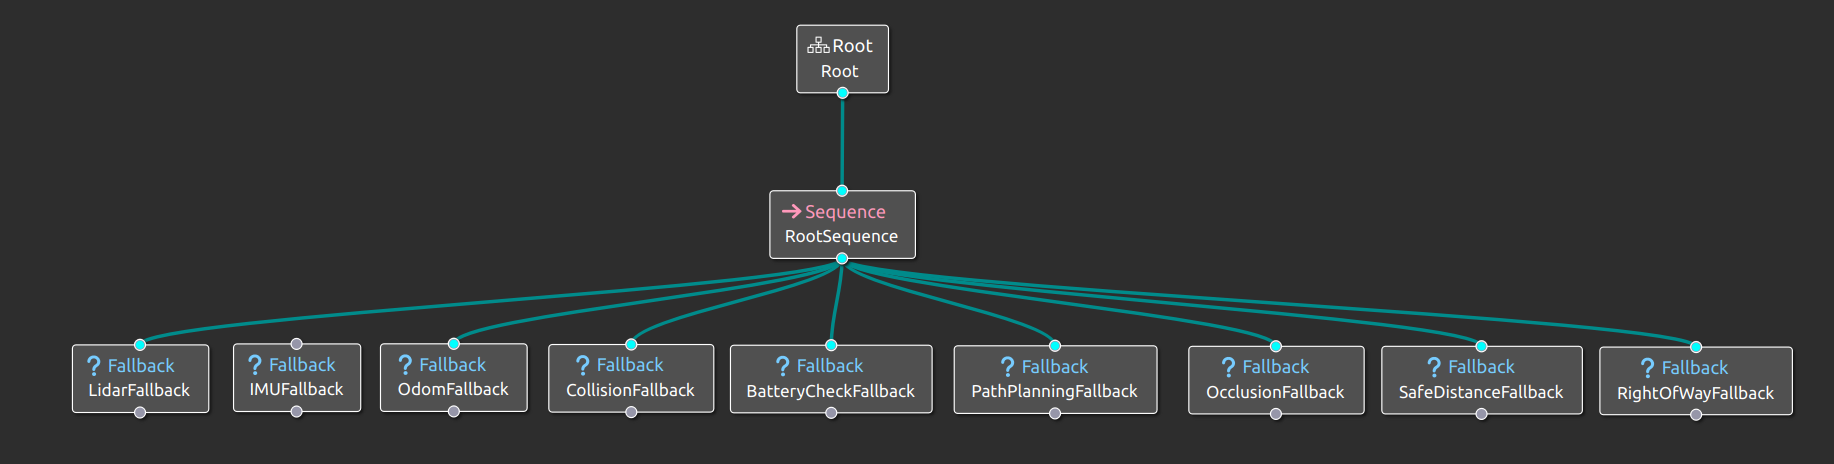
\includegraphics[width=1.0\textwidth]{images/simplified_bt.png}
	\caption{Top Level Behavior Tree Structure}
\end{figure}

\subsection{BT System Supervision}

The system supervisor component is partly outsourced into a component outside of the thread of the BT, because of the same reasons as the sensor backup component discussed in the previous section. The synchronous executor would stop the execution of the whole behavior tree, which is why the component needs to be moved inside of a new thread. The system supervisor, nachfolgend also called execution checker, is receiving messages from nodes that are not implemented as ROS2 lifecycle nodes. If a node stops sending messages or stops responding completely the external execution checker can inform the BT via a provided service of a problem with the node. ROS2 lifecycle nodes provide information about their health via an implementation of a FSM inside of the node. The current node state can be found out via a service call. However, to ensure the node is working correctly the output of the node needs to be checked too, because it might be that the FSM inside of the node did not pick up on a error. 
The system supervision is constantly checking the system's health. The BT is using service calls to get the health information about the compononts which are checked inside of Condition Nodes. 
The components get checked by the BT inside of a Fallback. If the condition for the execution is met, the Condition Node returns "success" and the fallback would exit to move on to the next fallback and execution condition check (see fig. xx). In case the execution checker detects a node failure, a sequence to react to the sensor failure is executed in which the robot slows down to a minimum and tries to restart the sensor. Should the restart fail the robot will not be able to navigate in a safe manner anymore and will come to a complete stop. This behavior pattern is realized for the lidar, the IMU and the wheel odometry. \\

\begin{figure}[h!]
	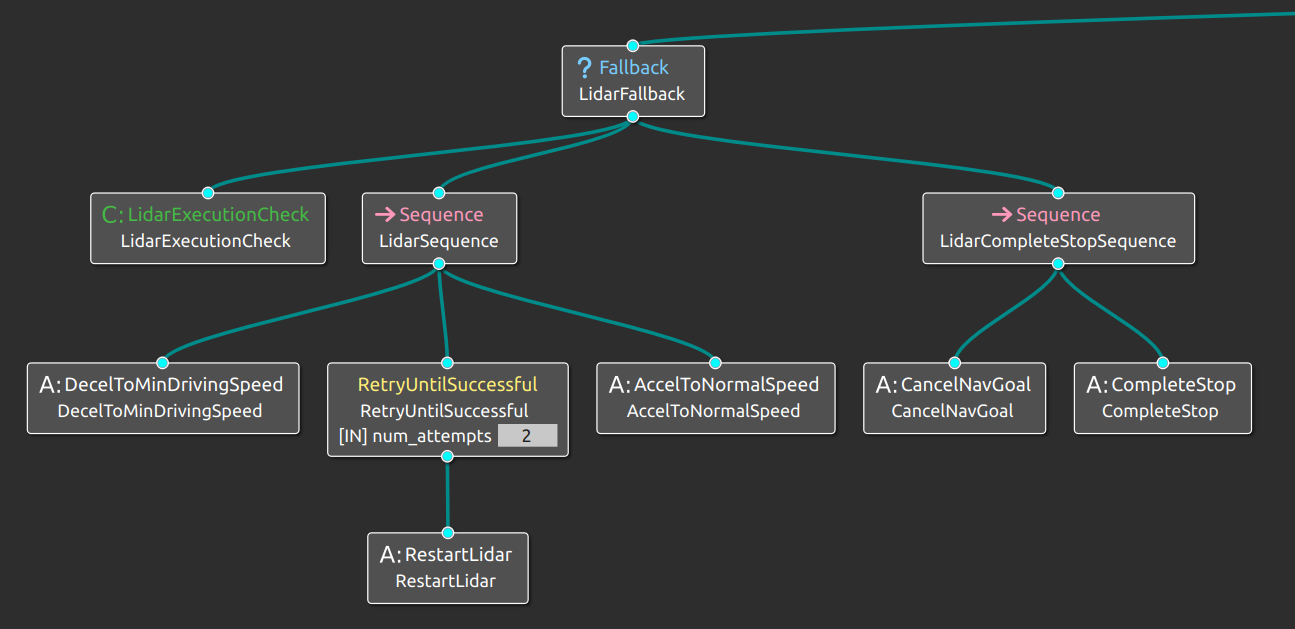
\includegraphics[width=1.0\textwidth]{images/sensor_fallback.png}
	\caption{Lidar Fallback}
\end{figure}

The timeout period for the execution checker to declare a node failed after no message was received is set at one second. 
After that period the goal is to enable to robot to continue to make progress towards the goal but if the system can not restart the sensor in a short time after failure, the robot has to come to a stop as a sensor failure is a severe function loss for the robot.


\subsection{BT Advanced Behaviors}
After the BT has checked for sensor failures and can guarantee that the environment representation is accurate, the system can check for more complicated scenarios to improve the autonomy. 


\subsubsection{Collision Behavior}
One of the biggest problems mentioned in chapter 3.1 is the inability to react to collisions. The collision can happen due to inadequate sensory coverage for detecting obstacles or general sensor inadequacy which can not detect obstacles because of their shape or surface material. With a multitude of sensors covering all angles and heights and computer vision capabilities to detect obstacles collisions would be very unlikely. But even if the robot could perrfectly detect obstacles, it would still be vulnerable to outside pertubations like other robots driving into it, humans accidently touching the robot etc. . 
To combat this the robot must be able to first detect that a collision occured, get out of the collision state, update the map and reset all costmaps to generate a new path to the original goal. 

\begin{figure}
	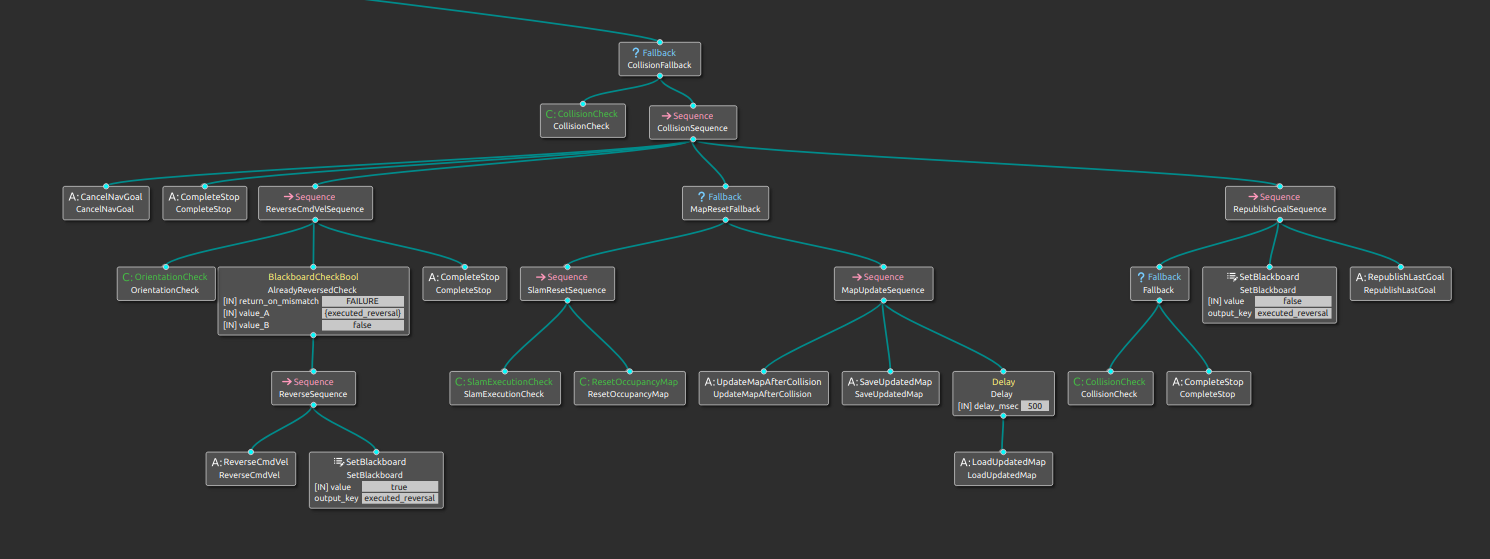
\includegraphics[width=1.0\textwidth]{images/collision_fallback.png}
	\caption{Collision Fallback Behavior}
\end{figure}

The collision checker uses a simulated sensor to detect collisions. On a real robot the collision checker can use a IMU-based collision detection, but this has not been implemented in this behavior tree due to time constraints of this thesis. The collision checker itself is integrated into the system supervisor and the BT is making service calls to the execution checker to get the collision state of the robot periodically. 
The child nodes of the collision sequence make use of the sensor data backup. 
To get out of the collision state, the BT requests the last saved command velocities from the data backup component and modifies them to reverse with minimum speed the same way the robot got into the collision. The reversing action takes longer than the two seconds as the commands get published with longer time intervals between them to adjust the driven distance to be the same as the navigation commands. An additional check is implemented before the reversing to make sure the robot only reverses once, otherwise the robot would be driving back and forth as the data backup service would provide the BT with the commands from the last reversing action. 

The modification is done in the following manner

\textit{Formula for determining execution time}

Regarding the map reset, we have to determine if we are creating a new map with a SLAM method or if the map server provided a previously saved map. 
In case of the running SLAM, the recent updates to the map must be verwerfen to a map prior to when the collision occurred.
When a static map is provided by the map server component from Nav2 the map needs to be updated with a new obstacle at the point of collision and republished by the map server. 

The activity of the "MapUpdateAfterCollision" action node is depicted in figure xx. The collision point is estimated by the robot's pose which refers to the robot base link and the robot footprint. We assumed that the collision point is right in front of the robot, because the local planner favours forward drive kinematics. The simulated bumper sensor can provide more nuanced information about the point of contact, but this functionality can not be achieved on a real robot with an IMU-based collsion detection, hence we simplified the obstacle position to always be in front of the robot. 
The collision position is calculated with 

\textit{Formula here}

A 25 by 25 cm square with full occupation of that space is added to the current map and then saved to be reloaded by the map server as depicted in figure xx. 

The original goal is then republished to replan the global path on the updated map. A more detailed view of the whole behavior is depicted in figure xx.

\begin{figure}
	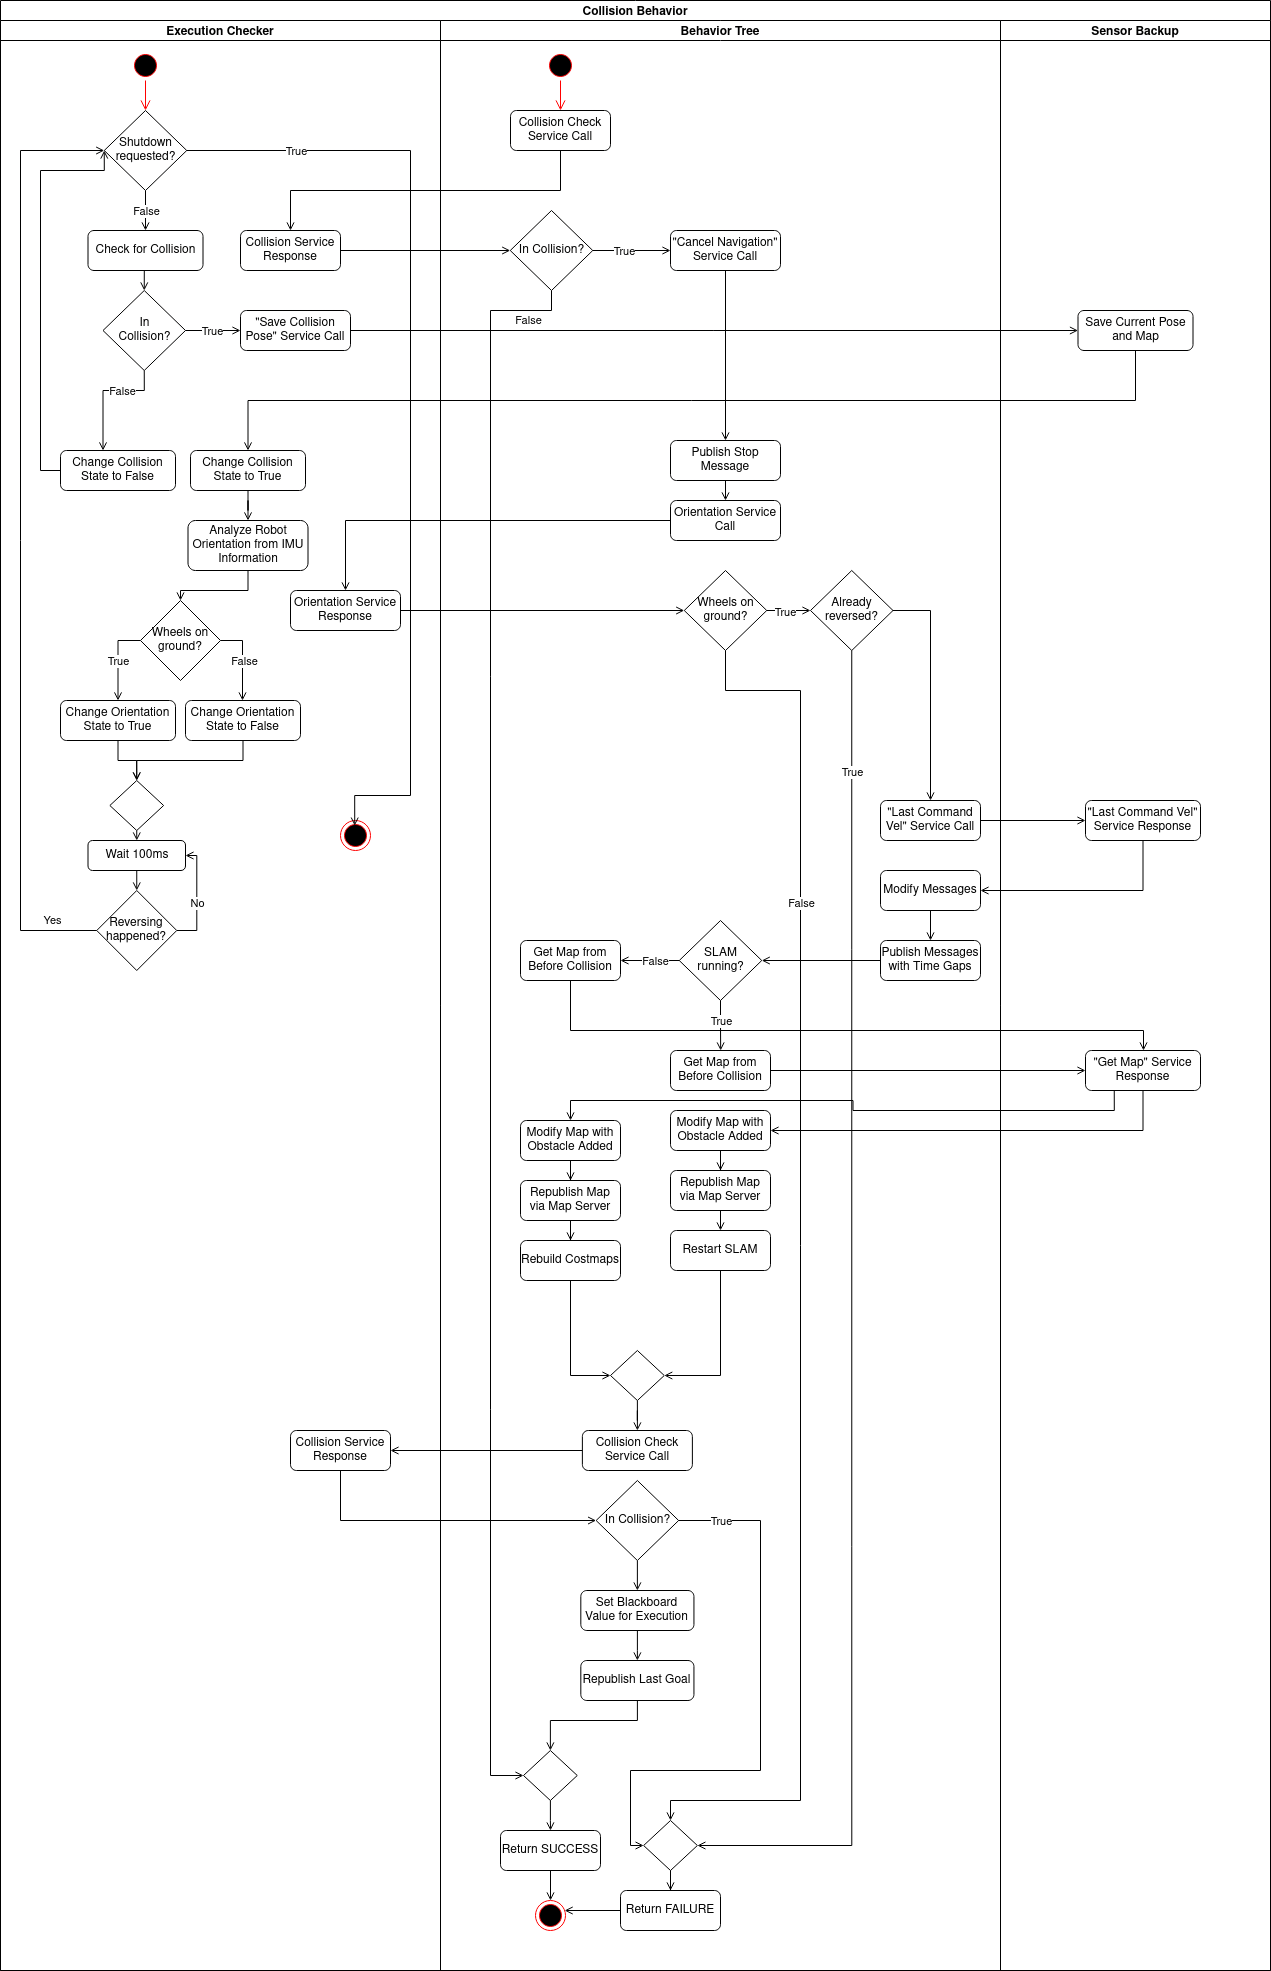
\includegraphics[width=0.9\textwidth]{images/activity_diagram_collision.png}
	\caption{Activity Diagram for the Collision Behavior}
\end{figure}

In this manner obstacles lower than the lidar scan height can be detected. With this behavior the robot should also be able to eventually navigate around transparent obstacles which do not reflect the laser. Glass doors are known to cause issues for robots based only on lidars. 

\subsubsection{Battery Behavior}

The battery behavior has the goal to monitor the robot's battery and has to make to the decision if the robot should navigate to a new goal location or not. The decision is based on the current battery charge and the estimated consumption of energy to reach the new goal. The robot should not begin the navigation process if it is probable that the remaining charge will not suffice for the driving.

\begin{figure}
	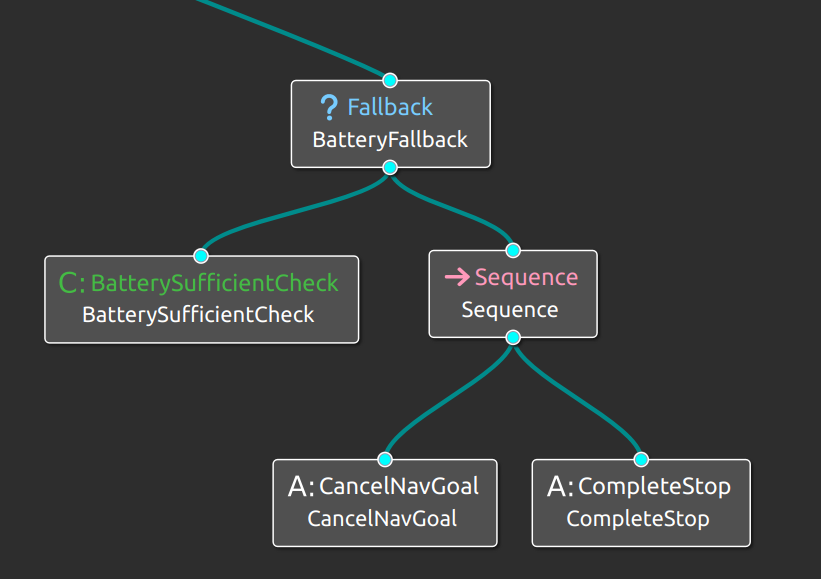
\includegraphics[width=0.5\textwidth]{images/battery_fallback.png}
	\caption{Battery Fallback Behavior}
\end{figure}
The robot has to take into account the idle consumption, the energy to drive the motors. With this information we created a simple linear function for the energy expenditure to predict the required power depending on the length of the path. To make the algorithm fail safe, we added an additional safety factor into the function, to berücksichtigen the scenario where the robot has to reroute and drive a longer route or has to stop for a moment. The resulting function can be described as: \\

\textit{Formel here}

On a real robot the average values for the idle and driving consumption could be experimentally determined. For the simulated turtlebot we created a simulated battery package which updates the battery charge every second. The battery package subscribes to the comman velocity topic and decreases the battery charge for every message that is received. We created the battery package because the behavior for this scenario needs to be tested. This is way the consumption rates are not close to reality.
The battery package provides a service to get the battery charge and the values for the angenommenen consumption rates. The BT node "IsBatterySufficientCheck" calls the service to compare the current battery to the calculated consumption. The battery behavior fallback will cancel the navigation goal if the robot can not reach the given goal with the remaining charge. \\

\subsubsection{Path Planning Behavior}

With this behavior, we implement a way to make the global planner more flexible. 
The execution checker component monitors the health of the Nav2 global planner. Additionally, the BT analyses the global planners output. If one of the condition fails, the given navigation goal is not reachable by the planning algorithm. We combat this by shifting the goal to a nearby alternative to get the robot as close to the original goal as possible. Is the location still unreachable, the goal gets moved further away and closer to the robot again. This routine gets repeated for up to ten times, which leads to a distance to the original goal of up to one meter. 
The goal gets moved on a straight vector towards the robot. Other strategies for finding alternative goals were not implemented in this behavior.


\begin{figure}[h!]
	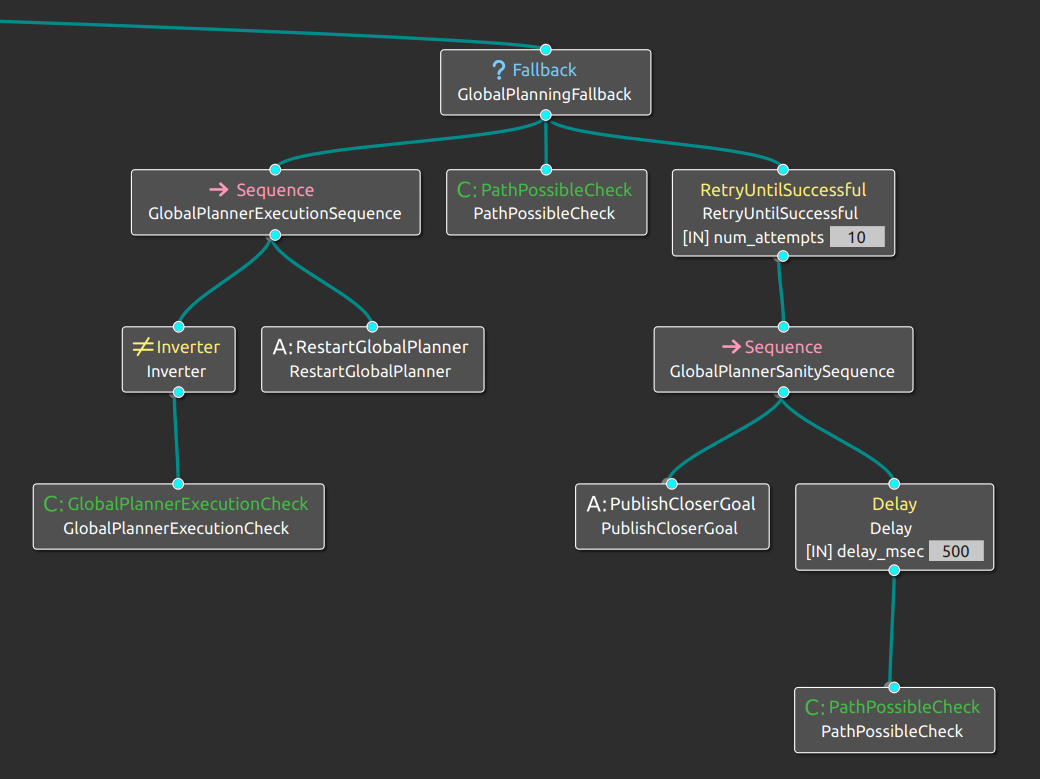
\includegraphics[width=0.7\textwidth]{images/global_planning_fallback.png}
	\caption{Path Planning Fallback Behavior}
\end{figure}



\section{System Support Tools}
\subsection{Gazebo Sensor Drivers}
For testing purposes, the simulated sensor data is not published directly on to the actual topic by gazebo. To control the flow of information in the system, an intermediary node is used, which subscribes to the Gazebo topic and republishes the information on the original topic. With this methodology, the failure of a sensor can be simulated as the simulation does not offer this functionality. Figure xx shows the RQT graph, which depicts the ROS nodes and their subscribed/published topics. 

\begin{figure}
	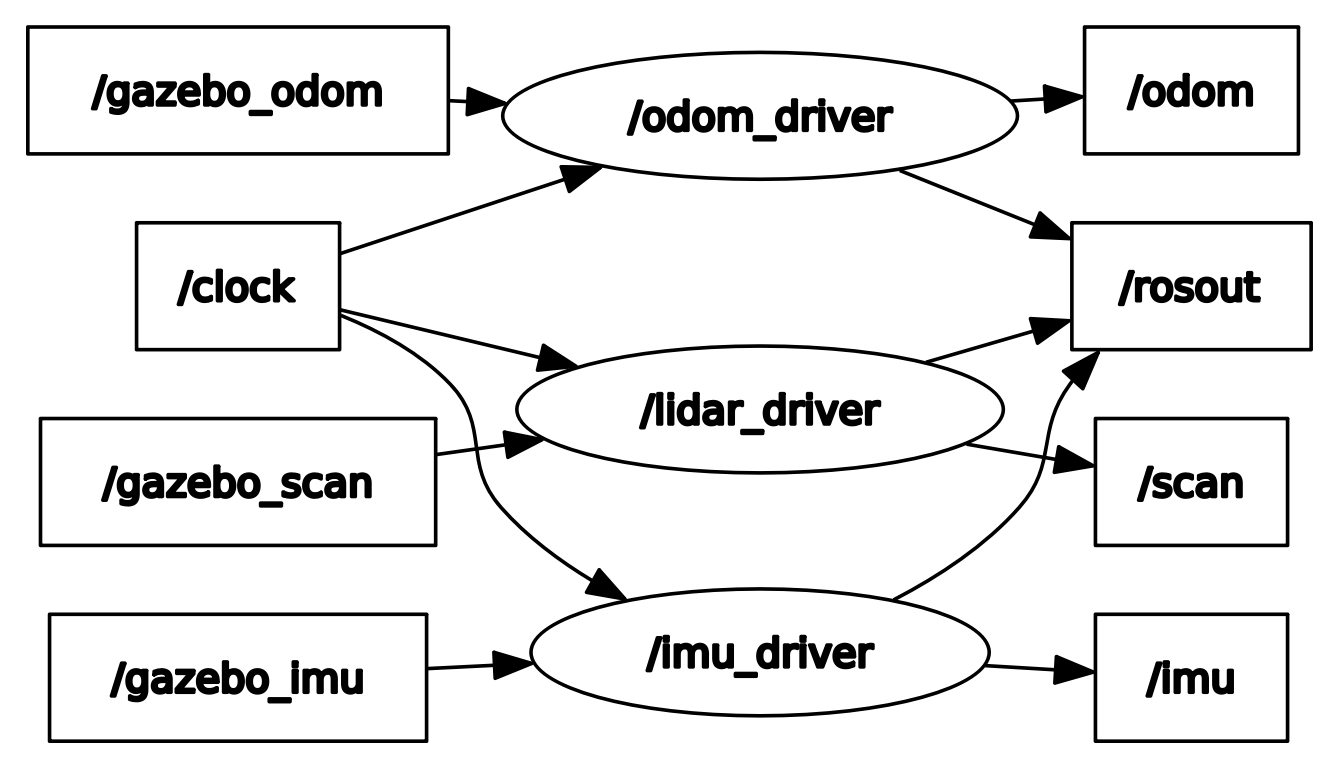
\includegraphics[width=0.75\textwidth]{images/rqt_graph_sensor_drivers.png}
	\caption{Graph for the Sensor Driver nodes and topics}
\end{figure}


\subsection{Custom ROS Interfaces}

Because of the neccessity to have ROS nodes spinning outside of the BT thread as discussed in 4.4.1, additional interfaces needed to be created in order to receive informations through service calls. The created service types are listed in table xx. All of the service definitions are created in a dedicated package named "bt$\_$msgs". 

\begin{table}[h!]
	\caption{Implemented Custom Services}
	\begin{tabular}{ | m{0.2\textwidth} | m{0.33\textwidth}| m{0.33\textwidth} | m{0.2\textwidth} |} 
  	\hline
  	Name & Request & Response \\ 
  	\hline
  	GetCharge & Empty & float charge, float idle$\_$decrease$\_$per$\_$sec, float drive$\_$decrease$\_$per$\_$sec \\
  	\hline
  	GetDistance & Empty & float distance$\_$in$\_$meter\\ 
  	\hline
  	GetLastGoal & Empty & geometry$\_$msgs/Pose last$\_$goal$\_$pose \\ 
  	\hline
  	GetLastMap & Empty & nav$\_$msgs/OccupancyGrid map \\
  	\hline
  	GetTwistArray & Empty & geometry$\_$msgs/Twist[] cmd$\_$vel$\_$array\\
  	\hline  	
  	PubCmdVel & geometry$\_$msgs/Twist cmd$\_$vel, float time$\_$in$\_$seconds & bool success \\
  	\hline
  	SendUpdatedMap & nav$\_$msgs/OccupancyGrid updated$\_$map & Empty \\
  	\hline
	\end{tabular}
\end{table}





